\documentclass[apj, revtex4]{emulateapj}

\usepackage{epsf}
\usepackage{color}
\usepackage{amsmath}
\usepackage{graphicx}
\usepackage[colorlinks,urlcolor=blue,citecolor=blue,linkcolor=blue]{hyperref}
\usepackage{threeparttable}
\usepackage{multirow}
\usepackage{natbib}
\usepackage{etoolbox}

\bibliographystyle{apj}
\citestyle{aa}
 
% General commands that are good for any agronomy paper.
%%% Fields %%%
\newcommand{\hdf}{HDF-N}
\newcommand{\hdfn}{HDF-N}
\newcommand{\hdfs}{HDF-S}
\newcommand{\cdfs}{CDF-S}

%%% Telescopes %%%
\newcommand{\hst}{\textit{HST}}
\newcommand{\iras}{\textit{IRAS}}
\newcommand{\iso}{\textit{ISO}}
\newcommand{\spitzer}{\textit{Spitzer}}
\newcommand{\sirtf}{\textit{Spitzer}}
\newcommand{\chandra}{\textit{Chandra}}

%%% Filters %%%
\newcommand{\wfu}{\hbox{$\mathrm{U}_{300}$}}
\newcommand{\wfb}{\hbox{$\mathrm{B}_{450}$}}
\newcommand{\wfv}{\hbox{$\mathrm{V}_{606}$}}
\newcommand{\wfi}{\hbox{$\mathrm{I}_{814}$}}
\newcommand{\acsb}{\hbox{$\mathrm{B}_{435}$}}
\newcommand{\acsv}{\hbox{$\mathrm{V}_{606}$}}
\newcommand{\acsi}{\hbox{$i_{775}$}}
\newcommand{\acsz}{\hbox{$z_{850}$}}
\newcommand{\nicj}{\hbox{$\mathrm{J}_{110}$}}
\newcommand{\nich}{\hbox{$\mathrm{H}_{160}$}}
\newcommand{\wfcy}{\hbox{$\mathrm{Y}_{105}$}}
\newcommand{\wfcj}{\hbox{$\mathrm{J}_{125}$}}
%\newcommand{\wfcj}{\hbox{$J_{110}$}}
\newcommand{\wfch}{\hbox{$\mathrm{H}_{160}$}}
\newcommand{\sdssu}{\hbox{$u$}}
\newcommand{\sdssg}{\hbox{$g$}}
\newcommand{\sdssr}{\hbox{$r$}}
\newcommand{\sdssi}{\hbox{$i$}}
\newcommand{\sdssz}{\hbox{$z$}}
\newcommand{\mone}{\hbox{$[3.6]$}}
\newcommand{\mtwo}{\hbox{$[4.5]$}}
\newcommand{\mthree}{\hbox{$[5.8]$}}
\newcommand{\mfour}{\hbox{$[8.0]$}}
%\newcommand{\mone}{\hbox{$[3.6\mu\mathrm{m}]$}}
%\newcommand{\mtwo}{\hbox{$[4.5\mu\mathrm{m}]$}}
%\newcommand{\mthree}{\hbox{$[5.8\mu\mathrm{m}]$}}
%\newcommand{\mfour}{\hbox{$[8.0\mu\mathrm{m}]$}}

%%% Astronomy Abreviations %%%
\newcommand{\mstar}{\hbox{$\mathrm{M}^\ast$}}
\newcommand{\lstar}{\hbox{$L^\ast$}}
\newcommand{\Msol}{\hbox{$\mathrm{M}_\odot$}}
\newcommand{\msol}{\hbox{$\mathrm{M}_\odot$}}
\newcommand{\Zsol}{\hbox{$Z_\odot$}}
\newcommand{\zsol}{\hbox{$Z_\odot$}}
\newcommand{\Lsol}{\hbox{$L_\odot$}}
\newcommand{\lsol}{\hbox{$L_\odot$}}
\newcommand{\lir}{\hbox{$L_{\mathrm{IR}}$}}
\newcommand{\zph}{\hbox{$z_\mathrm{ph}$}}
\newcommand{\zphot}{\hbox{$z_\mathrm{ph}$}}
\newcommand{\lbol}{\hbox{$L_\mathrm{bol}$}}
\newcommand{\snr}{\hbox{$\mathrm{S/N}$}}
\newcommand{\reff}{\hbox{$r_\mathrm{eff}$}}
\newcommand{\ks}{\hbox{$K_s$}}
\newcommand{\AAA}{\hbox{\AA}}

%%% Spectrum Lines %%%
\newcommand{\lya}{ Ly$\alpha \;$}
\newcommand{\lyb}{Lyman~$\beta$}
\newcommand{\hb}{\hbox{H$\beta$}}
\newcommand{\ha}{\hbox{H$\alpha$}}
\newcommand{\paa}{\hbox{Pa$\alpha$}}

%%% Units %%%
\newcommand{\kms}{\hbox{km~s$^{-1}$}}
\newcommand{\cms}{\hbox{cm~s$^{-1}$}}
\newcommand{\mpc}{\hbox{Mpc$^{-1}$}}
\newcommand{\mpcsq}{\hbox{Mpc$^{-2}$}}
\newcommand{\mpccu}{\hbox{Mpc$^{-3}$}}
\newcommand{\cnts}{\hbox{cnt~s$^{-1}$}} 
\newcommand{\cmsq}{\hbox{cm$^{-2}$}}
\newcommand{\cmcu}{\hbox{cm$^{-3}$}}
\newcommand{\ergscm}{\hbox{erg~s$^{-1}$~cm$^{-2}$}}
\newcommand{\uJy}{\hbox{$\mu$Jy}}
\newcommand{\ujy}{\hbox{$\mu$Jy}}
\newcommand{\degree}{\hbox{$^\circ$}}
\newcommand{\degsq}{\hbox{degree$^2$}}
\newcommand{\arcminsq}{\hbox{arcmin$^2$}}
\newcommand{\um}{\hbox{$\mu$m}}

%%% Math %%%
\newcommand{\lsim}{\lesssim}
\newcommand{\gsim}{\gtrsim}
\newcommand{\mathS}{\hbox{$\mathcal{S}$}}
\newcommand{\mathR}{\hbox{$\mathcal{R}$}}
\newcommand{\mathM}{\hbox{$\mathcal{M}$}}
\newcommand{\mcal}{\hbox{$\mathcal{M}$}}
\newcommand{\rcal}{\hbox{$\mathcal{R}$}}
\newcommand{\scal}{\hbox{$\mathcal{S}$}}
\newcommand{\infinity}{\hbox{$\infty$}}
\newcommand{\err}[2]{$^{+#2}_{-#1}$}

%%% General %%%
\newcommand{\etal}{et al.}
\newcommand{\eg}{e.g.}
\newcommand{\ie}{i.e.}
\newcommand{\cf}{cf.}
% \newcommand{\ion}[2]{\hbox{#1$\;${\small\rm{#2}}}}
\newcommand{\mybullet}{\noindent$\bullet$}
\newcommand{\uit}{\textit{UIT}}
\newcommand{\nd}{...}
%\newcommand{\cmodel}{\hbox{\tt cmodel}}
%\newcommand{\bs}{\hbox{$\!\!\!\!$}}
\newcommand{\todo}[1]{{\tt #1}}
\newcommand{\citeeg}[1]{(\eg, \citealt{#1})}
\newcommand{\ignore}[1]{}

%%% Extra %%% 
% \newcommand{\farcm}{\mbox{\ensuremath{.\mkern-4mu^\prime}}}%fractional arcminute symbol 0.'0
% \newcommand{\farcs}{\mbox{\ensuremath{.\!\!^{\prime\prime}}}}%fractional arcsecond symbol: 0.''0
% \newcommand{\fdg}{\mbox{\ensuremath{.\!\!^\circ}}}%fractional degree symbol:     0.°0
\newcommand{\arcdeg}{\ensuremath{^{\circ}}}%                    % degree symbol:  °
% \newcommand{\sun}{\ensuremath{\odot}}%                          % sun symbol
% \newcommand{\apj}{ApJ}%                                         % Journal abbreviations
% \newcommand{\apjs}{ApJS}
% \newcommand{\apjl}{ApJL}
% \newcommand{\aap}{A{\&}A}
% \newcommand{\aaps}{A{\&}AS}
% \newcommand{\mnras}{MNRAS}
% \newcommand{\aj}{AJ}
% \newcommand{\araa}{ARAA}
% \newcommand{\pasp}{PASP}
\newcommand{\Teff}{\ensuremath{T_{\mathrm{eff}}}}%              % T_eff
\newcommand{\logg}{\ensuremath{\log g}}%                        % log g
\newcommand{\bv}{\ensuremath{B\!-\!V}}%                         % B-V
\newcommand{\ub}{\ensuremath{U\!-\!B}}%                         % U-B
\newcommand{\vr}{\ensuremath{V\!-\!R}}%                         % V-R
\newcommand{\ur}{\ensuremath{U\!-\!R}}%                         % U-R

\makeatletter
% Patch case where name and year are separated by aysep
\patchcmd{\NAT@citex}
  {\@citea\NAT@hyper@{%
     \NAT@nmfmt{\NAT@nm}%
     \hyper@natlinkbreak{\NAT@aysep\NAT@spacechar}{\@citeb\@extra@b@citeb}%
     \NAT@date}}
  {\@citea\NAT@nmfmt{\NAT@nm}%
   \NAT@aysep\NAT@spacechar\NAT@hyper@{\NAT@date}}{}{}

% Patch case where name and year are separated by opening bracket
\patchcmd{\NAT@citex}
  {\@citea\NAT@hyper@{%
     \NAT@nmfmt{\NAT@nm}%
     \hyper@natlinkbreak{\NAT@spacechar\NAT@@open\if*#1*\else#1\NAT@spacechar\fi}%
       {\@citeb\@extra@b@citeb}%
     \NAT@date}}
  {\@citea\NAT@nmfmt{\NAT@nm}%
   \NAT@spacechar\NAT@@open\if*#1*\else#1\NAT@spacechar\fi\NAT@hyper@{\NAT@date}}


%Commands specific to the this work
\newcommand{\editorial}[1]{\textcolor{red}{#1} }
\DeclareRobustCommand{\ion}[2]{%
\relax\ifmmode
\ifx\testbx\f@series
{\mathbf{#1\,\mathsc{#2}}}\else
{\mathrm{#1\,\mathsc{#2}}}\fi
\else\textup{#1\,{\mdseries\textsc{#2}}}%
\fi}

%-----------------------------------------------------------------------------------------

\shorttitle{Cluster Paper}
\shortauthors{BOADA ET AL.}

%\slugcomment{\it Draft Version \today}
%\slugcomment{\it Submitted for publication in the Astrophysical Journal}
%\slugcomment{Accepted for Publication in the Astrophysical Journal}

\begin{document}

\title{Cluster Paper}

\author{\sc Steven Boada\altaffilmark{1}, 
C.~Papovich\altaffilmark{1},
B.~Salmon\altaffilmark{1}, 
N.~Merhtens\altaffilmark{1},
T.~Li\altaffilmark{1}, 
R.~Wechsler\altaffilmark{2,3},
E.~Rozo\altaffilmark{2,4},
E.~Rykoff\altaffilmark{2,5}} 

\altaffiltext{1}{George P.\ and Cynthia Woods Mitchell Institute for
Fundamental Physics and Astronomy, and Department of Physics and Astronomy,
Texas A\&M University, College Station, TX, 77843-4242;
boada@physics.tamu.edu}
\altaffiltext{2}{Kavli Institute for Particle Astrophysics and Cosmology, Department of Physics, Stanford University, Stanford, CA 94305, USA}
\altaffiltext{3}{Department of Particle Physics and Astrophysics, SLAC National Accelerator Laboratory, Menlo Park, CA 94025, USA}
\altaffiltext{4}{Department of Astronomy, University of Chicago, Chicago, IL 60637, USA}
\altaffiltext{5}{E. O. Lawrence Berkeley National Lab, 1 Cyclotron Road, Berkeley, CA 94720, USA}

\begin{abstract}
\noindent
ABSTRACT GOES HERE!!
Lorem ipsum dolor sit amet, consectetur adipisicing elit, sed do eiusmod tempor incididunt ut labore et dolore magna aliqua. Ut enim ad minim veniam, quis nostrud exercitation ullamco laboris nisi ut aliquip ex ea commodo consequat. Duis aute irure dolor in reprehenderit in voluptate velit esse cillum dolore eu fugiat nulla pariatur. Excepteur sint occaecat cupidatat non proident, sunt in culpa qui officia deserunt mollit anim id est laborum.
\end{abstract}

\section{INTRODUCTION}

\section{AARDVARK SIMULATION}
\editorial{Waiting to get a look at what Casey comes up with for the proposal we are supposedly writing. If he does a decent job then I'll try to expand it a bit and fill out this section.}
\begin{figure} 
	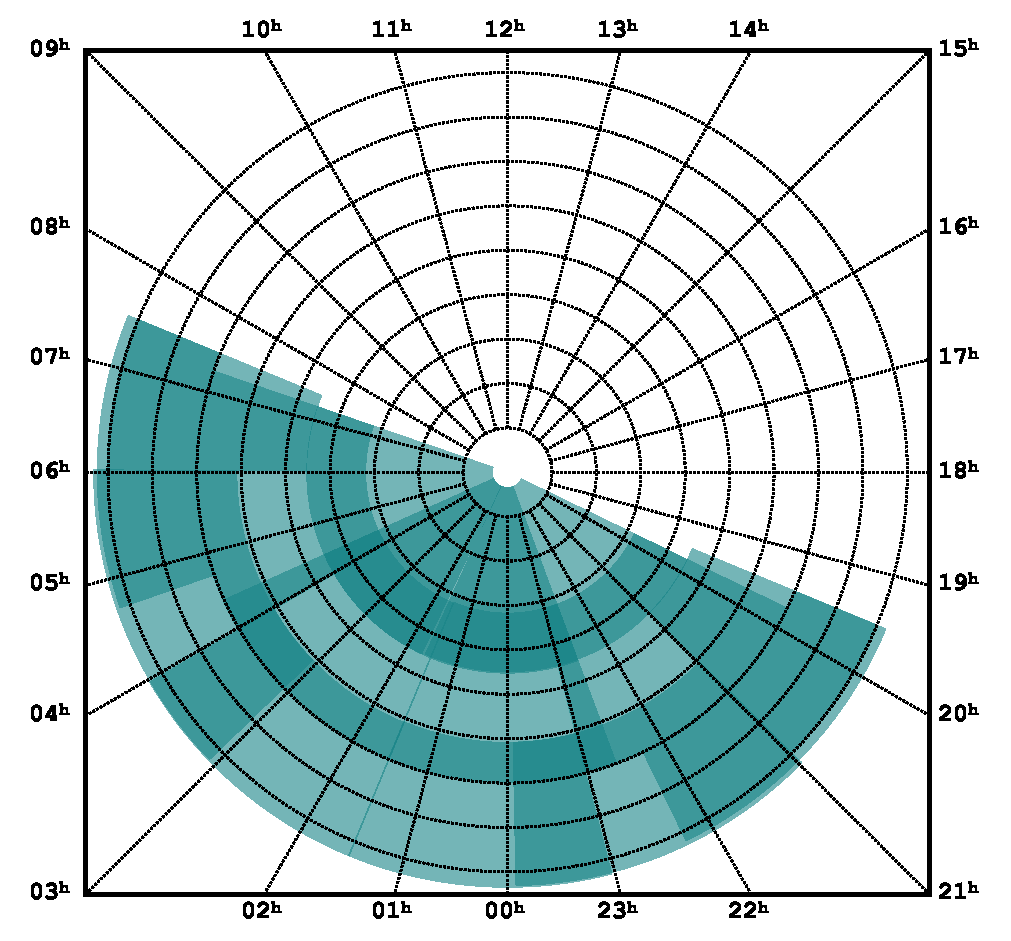
\includegraphics[width=0.49\textwidth]{surveyArea.pdf} 
	\caption{A polar azimuthal equidistant projection of the southern sky showing the sky area (approximately a quarter of the sky) covered by the Aardvark Simulations. Concentric circles are lines of constant declination, 10 to $-80\degree$ in $10\degree$ increments. Radial lines are lines of constant right ascension. Opaqueness of the region indicates the overlap of catalog tiles (see text for details).} 
	\label{fig:survey area} 
\end{figure}

\section{THE HETDEX SURVEY}
\editorial{This should probably go into the introduction. I don't think we need a whole section on something that a bunch of papers have already talked about.}

\section{Mock Observations}
\editorial{Here we need to talk about about how we set up the observations to look like what we think the HETDEX survey will see. It should be more technical than the general discussion about what the survey hopes to accomplish, that'll go in the intro. A zoomed figure showing the tiling footprints would be appropriate.}

\begin{figure} 
	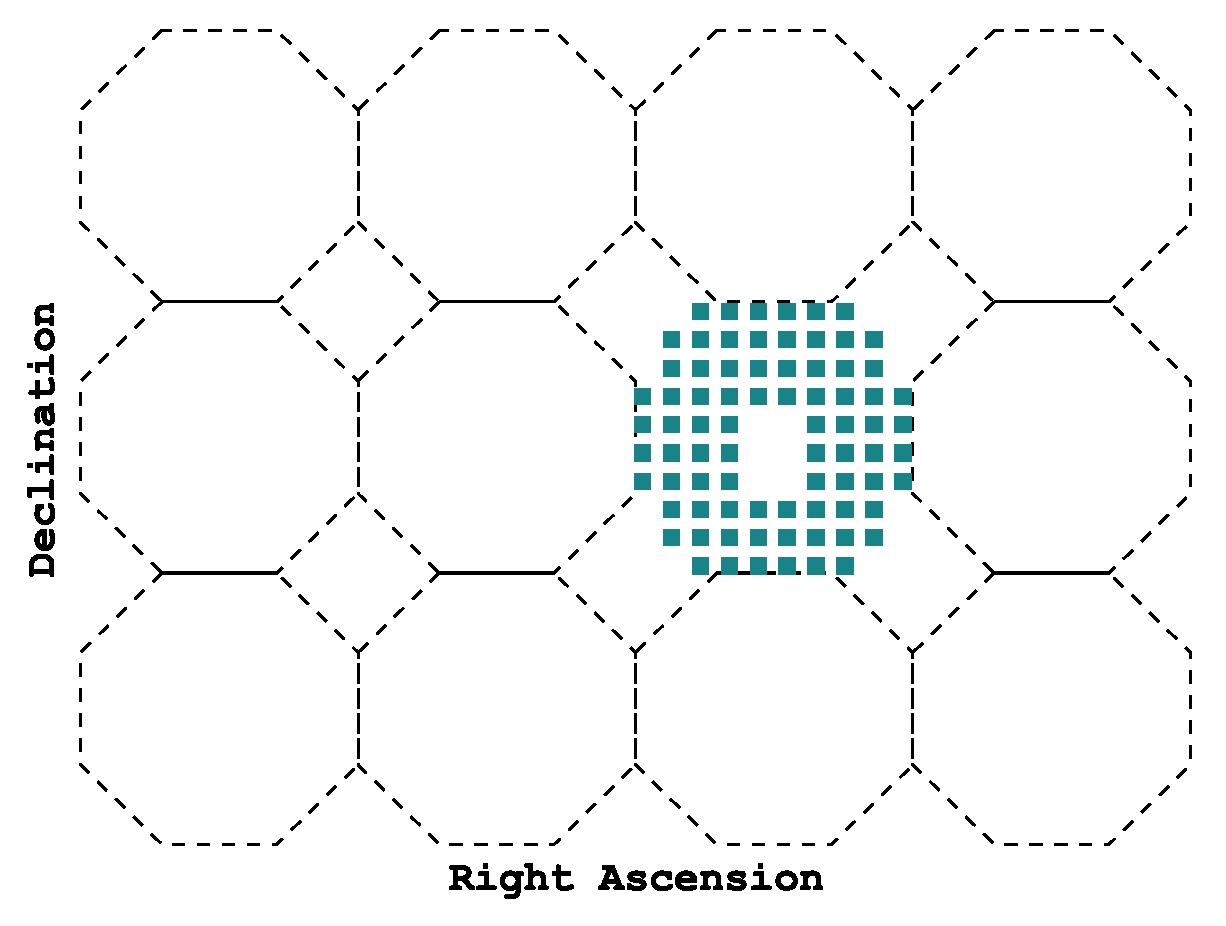
\includegraphics[width=0.49\textwidth]{f01.pdf} 
	\caption{} \label{fig:ifu layout} 
\end{figure}

\section{Recovery of Cluster Parameters, Full Knowledge}

Lorem ipsum dolor sit amet, consectetur adipisicing elit, sed do eiusmod tempor incididunt ut labore et dolore magna aliqua. Ut enim ad minim veniam, quis nostrud exercitation ullamco laboris nisi ut aliquip ex ea commodo consequat. Duis aute irure dolor in reprehenderit in voluptate velit esse cillum dolore eu fugiat nulla pariatur. Excepteur sint occaecat cupidatat non proident, sunt in culpa qui officia deserunt mollit anim id est laborum.

\subsection{Cluster Redshift}
The accurate determination of the cluster redshift ($z_c$) is crucial to the reliability of all following measurements. An incorrect cluster redshift introduces errors into the measured line of sight velocity (LOSV) and corresponding dispersion, which, in turn, contributes to errors associated with dynamical mass and radius. 

In simple terms, the cluster redshift is the  mean of the redshifts of all galaxies associated with the cluster. However, because the standard mean can be quite sensitive to outliers or otherwise contaminated data, we require a more resistant statistic, and turn to the biweight location estimator \citep{Beers1990} which provides improved performance. 

We compare the calculated cluster redshifts to the true redshift ($z_{c,true}$) for 107748 galaxies comprising 1683 unique halos, and we find a RMS$[\delta z/(1+z_{c,true})]= 4\times 10^{-4}$ where $\delta z = z_{c,true} - z_{c}$. 

\editorial{The RMS using just the regular mean is 3.8e-4 which is only slightly better than the biweight. I don't think that will be the case when we get more complicated things.}

\subsection{Line of Sight Velocity Dispersion}
The unbiased estimation of a standard deviation (a measure of statistical dispersion) is a technically involved problem. At first, we require that our estimator be unbiased in that the dispersion estimation is equal to the true dispersion, although, in practice this rarely occurs. The most commonly used estimate is the corrected sample standard deviation, given by:
\begin{equation}
	s = \sqrt{\frac{1}{n-1} \sum_{i=1}^n (x_i - \bar{x})^2}
\end{equation}
with $\{x_1, x_2, ..., x_n\}$ is the random sample and $\bar{x}$ is the sample mean. The corrected sample standard deviation has the advantage in that it is unbiased (as opposed to the population standard deviation which is biased), but the removal of bias relies on knowing \textit{a priori} the underlying distribution from which the sample is drawn. An estimator which correctly estimates a standard deviation for a sample drawn from a wide range of distributions and is not adversely effected by outliers is said to be \textit{robust}.

A robust estimator becomes critical as it minimizes the effect that outliers which may remain after the rejection of non-cluster members have on the measured dispersion. \cite{Beers1990} present a robust estimation of scale (yet another term for statistical dispersion) called the biweight scale estimator. \cite{Ruel2014} note that the biweight scale estimator is biased and suggest a correction. 

The biweight scale estimator is given by \editorial{This isn't very good and needs to be rewritten but it gets the idea across.}:
\begin{equation}
	\sigma_{BI} = \sqrt{ N_{members} \frac{ \sum_{|u_i|<1} (1-u_i^2)^4 (v_i - \bar{v})^2} {D} }
\end{equation}
with $v_i$, the proper velocities, $\bar{v}$, the average of the proper velocities,
\begin{equation}
	D = \sum_{|u_i|<1} (1-u_i^2)(1-5u_i^2)
\end{equation}
with $u_i$ being the biweight weighting and defined as:
\begin{equation}
	u_i = \frac{v_i - \bar{v}}{9 {\rm MAD}(v_i)}
\end{equation}
where MAD is the median absolute deviation.

\editorial{Need to talk about how the new biweight is different. Also need to talk about how we are using DM halos and not galaxies, so we are only going to do so well when comparing the 3d dispersions and the dispersions that we are calculating. Evrard2008 does a good job explaining the DM-galaxy bias we are assuming it is 1}

\subsection{Dynamical Mass}
Recently, the relationship between the velocity dispersion and dynamical mass has been the focus of several studies (\eg, \citealt{Evrard2008, Saro2013, Sifon2013, VanderBurg2014}), and find a best-fitting relation for the mass enclosed by $r_{200c}$ of the form
\begin{equation}
	M_{200c} = \frac{10^{15}}{h(z)} \bigg{(}\frac{\sigma_{1D}}{\sigma_{15}} \bigg{)}^{-\alpha} \Msol
\end{equation}
where $\sigma_{15} = 1082.9 \pm 4.0 \kms$, $\alpha = 0.3361 \pm 0.0026$, $h(z) = H_0 \sqrt{\Omega_\Lambda + (1+z)^3\Omega_M}$, and $\sigma_{1D}$ is the 1D velocity dispersion of the dark matter particles, which is related to the velocity dispersions of the galaxies. 

\editorial{Need to talk about how the parameters are some what up for debate, and vary from study to study. I think we should just use the params from Evrard2008 and call it a day. We can show a figure where we fit the data for the parameters, but that seems kinda silly to calibrate the data on the the data we are trying to fit.}

\subsection{Radial Extent}
\begin{equation}
	r_{200} = \bigg{[} \frac{3}{4\pi} \frac{M_{200}}{200\rho_c} \bigg{]}^{1/3}
\end{equation}

\section{Evidence of Substructure}
Lorem ipsum dolor sit amet, consectetur adipisicing elit, sed do eiusmod tempor incididunt ut labore et dolore magna aliqua. Ut enim ad minim veniam, quis nostrud exercitation ullamco laboris nisi ut aliquip ex ea commodo consequat. Duis aute irure dolor in reprehenderit in voluptate velit esse cillum dolore eu fugiat nulla pariatur. Excepteur sint occaecat cupidatat non proident, sunt in culpa qui officia deserunt mollit anim id est laborum.
\subsection{From VD profiles}
Lorem ipsum dolor sit amet, consectetur adipisicing elit, sed do eiusmod tempor incididunt ut labore et dolore magna aliqua. Ut enim ad minim veniam, quis nostrud exercitation ullamco laboris nisi ut aliquip ex ea commodo consequat. Duis aute irure dolor in reprehenderit in voluptate velit esse cillum dolore eu fugiat nulla pariatur. Excepteur sint occaecat cupidatat non proident, sunt in culpa qui officia deserunt mollit anim id est laborum.
\subsection{Mod-Dominance}
Lorem ipsum dolor sit amet, consectetur adipisicing elit, sed do eiusmod tempor incididunt ut labore et dolore magna aliqua. Ut enim ad minim veniam, quis nostrud exercitation ullamco laboris nisi ut aliquip ex ea commodo consequat. Duis aute irure dolor in reprehenderit in voluptate velit esse cillum dolore eu fugiat nulla pariatur. Excepteur sint occaecat cupidatat non proident, sunt in culpa qui officia deserunt mollit anim id est laborum.
\subsection{Dressler-Schectman Test}
We leverage the large spectroscopic dataset to study the structural properties of the clusters. \cite{Pinkney1996} determine, from a comparison of five different methods that the Dressler-Shectman (DS) test \citep{Dressler1988} is the most sensitive to the presence of substructure.

The DS test, which combines the spatial positions and velocities of the galaxies, provides a method to locate substructure by identifying groups of galaxies which differ significantly from the cluster velocity distribution. Galaxy subsets are selected from a cluster of $n_{members}$ and each constituent galaxy deviation is calculated according to
\begin{equation}
	\delta_i^2 = \frac{N_{local}+1}{\sigma^2}\bigg{[}(\bar{v}_{local,i} - \bar{v})^2 + (\sigma_{local,i} - \sigma)^2\bigg{]}^2
\end{equation}
where $\bar{v}_{local}$ and $\sigma_{local}$ are the mean velocity and velocity dispersion for a subset of $N_{local}$ galaxies and $\bar{v}$ and $\sigma$ are the entire cluster's mean velocity and velocity dispersion. The choice of $N_{local}$ is left to the user. Originally, \cite{Dressler1988} choose $N_{local}=10$, however \cite{Bird1994} points out that using a fixed value for $N_{local}$ reduces the sensitivity to substructure. We follow \cite{Bird1994} in choosing $N_{local} = \sqrt n_{members}$. \editorial{doesn't talk about the nearest neighbors which is what we are using.}

The DS statistic is the $\Delta$-value given by, 
\begin{equation}
	\Delta = \sum^{n_{members}}_i \delta_i
\end{equation}
where a system is considered to contain substructure if $\Delta/n_{members} > 1$ \citep{Dressler1988}. A second method, described in \cite{Hou2012}, uses probabilities (P-values) rather than a threshold for the identification of substructure. P-values are computed by comparing the observed $\Delta$-value and the $Delta$-value after the velocities (but not positions) have been shuffled through a series of Monte Carlo runs. The probability of the existence of substructure becomes
\begin{equation}
	P = \sum (\Delta_{shuffled} > \Delta_{Observed}) / n_{shuffle}
\end{equation}
where $n_{shuffle}$ is the number of shufflings used. \editorial{This sounds a whole lot like the description given in Hou2012. Make sure that we aren't copying anything word for word. That'd be bad.}

In practice, we use locate the nearest neighbors using an unsupervised k-nearest neighbor algorithm as implemented in Scikit-Learn \citep{Pedregosa2012}. 

\section{RESULTS}

\subsection{\ion{O}{ii} Luminosity}

HETDEX is designed to detect Lyman-$\alpha$ at redshift two. That allows us to detect \ion{O}{ii} emitters to $z\sim 0.49$. The catalog does not provide \ion{O}{ii} luminosities so we must assign them empirically. We use 177107 galaxies from the Sloan Digital Sky Survey (SDSS) Data Release 12 \citep{Alam2015} from $z = 0.05 - 0.2$. Galaxies are selected which have no redshift warning and have an \ion{O}{ii} flux five times greater than the \ion{O}{ii} flux error. 

\begin{figure} 
	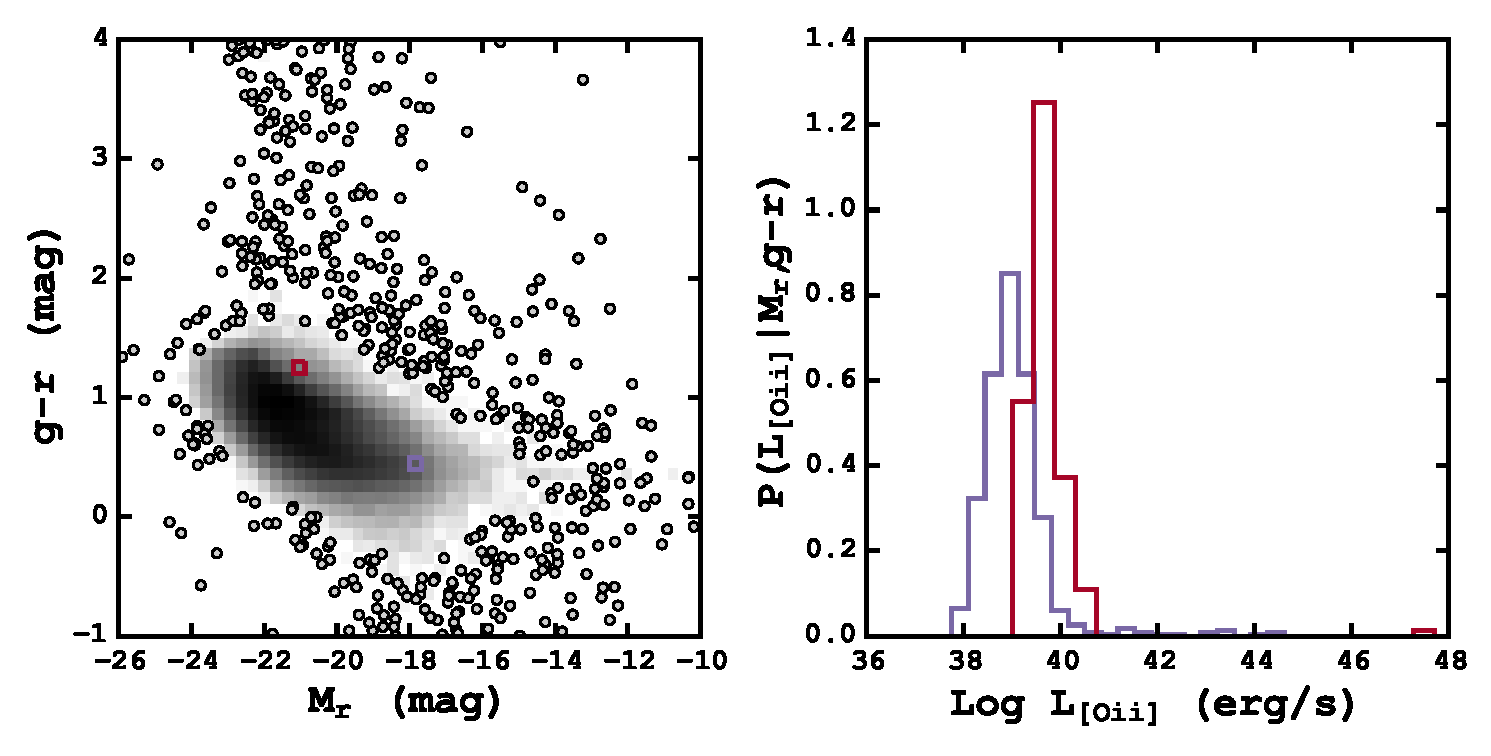
\includegraphics[width=0.49\textwidth]{oii_sdss.pdf} 
	\caption{} \label{fig:oii sdss} 
\end{figure}

We place each SDSS galaxy on a color-magnitude diagram (CMD) of $M_r$ and $g-r$, see Figure~\ref{fig:oii sdss}. To assign an \ion{O}{ii} luminosity to each galaxy in our catalog we place the galaxies on the same and select all SDSS galaxies in a small 2D bin around the galaxy. We extract all of the SDSS galaxies inside that bin and create a histogram of their \ion{O}{ii} luminosities. Using a slice sampling technique we assign the catalog galaxy an \ion{O}{ii} luminosity based on the distribution of SDSS galaxies extracted.

For catalog galaxies which are placed on the CMD near no, or very few ($n<3$) galaxies we assign it zero \ion{O}{ii} luminosity or the mean luminosity, respectively.

\section{IMPROVEMENT}
Lorem ipsum dolor sit amet, consectetur adipisicing elit, sed do eiusmod tempor incididunt ut labore et dolore magna aliqua. Ut enim ad minim veniam, quis nostrud exercitation ullamco laboris nisi ut aliquip ex ea commodo consequat. Duis aute irure dolor in reprehenderit in voluptate velit esse cillum dolore eu fugiat nulla pariatur. Excepteur sint occaecat cupidatat non proident, sunt in culpa qui officia deserunt mollit anim id est laborum.
\section{SUMMARY}
Lorem ipsum dolor sit amet, consectetur adipisicing elit, sed do eiusmod tempor incididunt ut labore et dolore magna aliqua. Ut enim ad minim veniam, quis nostrud exercitation ullamco laboris nisi ut aliquip ex ea commodo consequat. Duis aute irure dolor in reprehenderit in voluptate velit esse cillum dolore eu fugiat nulla pariatur. Excepteur sint occaecat cupidatat non proident, sunt in culpa qui officia deserunt mollit anim id est laborum.
\bibliography{master}

\end{document}